\documentclass[11pt]{article}
\usepackage[letterpaper,margin=1in]{geometry}
\usepackage{color}
\usepackage[dvipdfmx]{graphicx}
\usepackage{amsbsy}
\usepackage{amsmath}
\usepackage{adjustbox}
\usepackage{url}

\newcommand{\argmax}{\mathop{\rm arg~max}\limits}

\begin{document}
\vspace{-1cm}
\title{Analysis Report on Assignment 4: Boosting}
\vspace{-1cm}
\author{Yoshinari Fujinuma\vspace{-2ex}}
\date{\vspace{-2ex}}
\maketitle
\section{Boosting Iterations with Different Tree Depths}
\vspace{-0.6cm}
\begin{figure}[htb]
  \begin{center}
   \begin{tabular}{c}

    %\begin{minipage}{0.5\hsize}
    \begin{minipage}{0.3\hsize}
     \begin{center}
     %\scalebox{0.33}
     \scalebox{0.20}
      {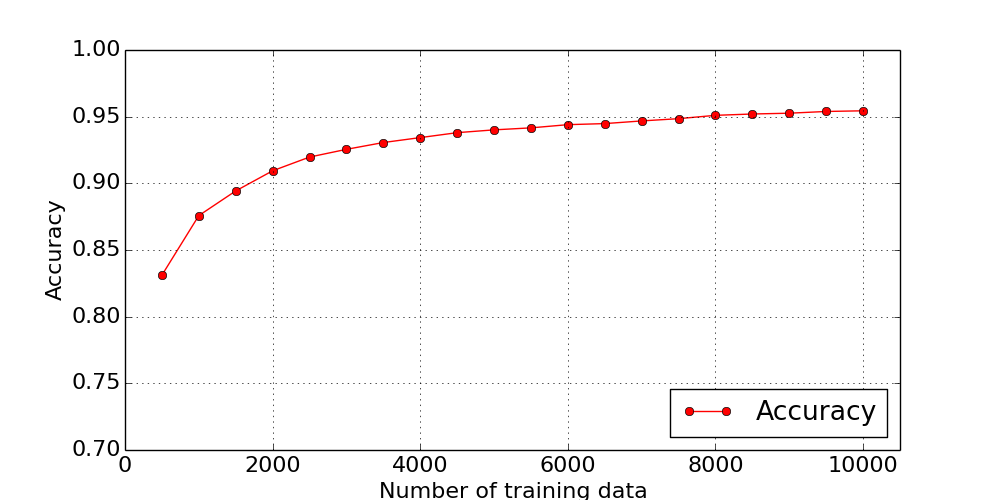
\includegraphics[]{figure_1.png}}
   
      \caption{\label{fig:1}Testing set and training set accuracy when tree depth$ = 1$.}
     \end{center}
    \end{minipage}

    \begin{minipage}{0.01\hsize}
    \end{minipage}

    %\begin{minipage}{0.5\hsize}
    \begin{minipage}{0.3\hsize}
     \begin{center}
      %\scalebox{0.33}
      \scalebox{0.20}
      {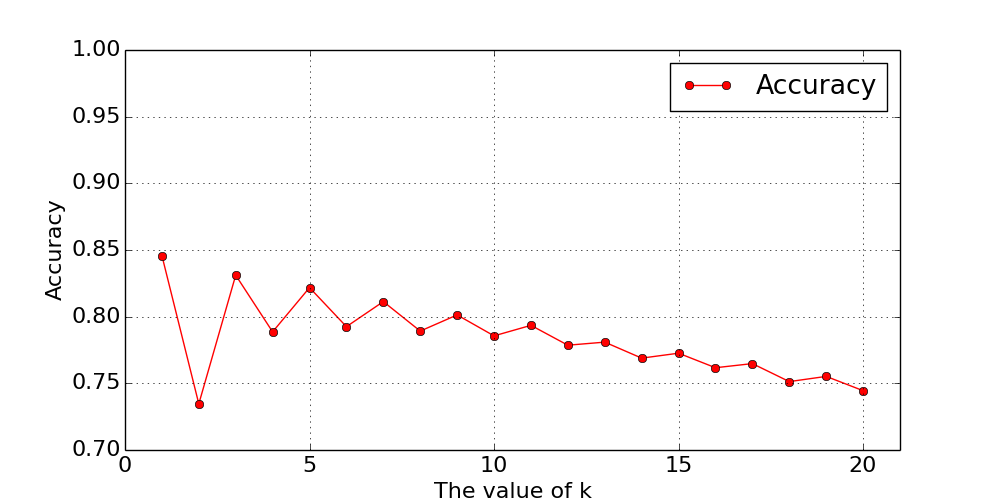
\includegraphics[]{figure_2.png}}
      \caption{Testing set and training set accuracy when tree depth$ = 2$.}
     \end{center}
    \end{minipage}

    \begin{minipage}{0.01\hsize}
    \end{minipage}

    \begin{minipage}{0.3\hsize}
     \begin{center}
      %\scalebox{0.33}
     \scalebox{0.20}
      {\includegraphics[]{figure_3.png}}
      \caption{Testing set and training set accuracy when tree depth$ = 3$.}
     \end{center}
    \end{minipage}



  \end{tabular}
 \end{center}
\vspace{-0.4cm}
\end{figure}

Figure \ref{fig:1} shows that the ensemble of depth $1$ trees shows a slight underfitting. $700$ iterations are not enough although the increase in training set accuracy is slightly limited. 
As the depth of each tree increases, the more it overfits in general. This is apparent when the depth of the tree is $3$. After it hits the test set accuracy of $0.990$ around the $400$th iteration, the accuracy gradually decreases. Also note that during that time, the training set accuracy is $1.0$.

\section{Boosting Iterations with Perceptron}
\vspace{-0.6cm}
\begin{figure}[htb]
  \begin{center}

   \begin{tabular}{c}
    \begin{minipage}{0.5\hsize}
     \begin{center}
     \scalebox{0.33}
      {\includegraphics[]{figure_4.png}}
      \caption{\label{fig:4}Testing set and training set accuracy when Perceptron as the base learner. The parameter $n\_iter$ for Perceptron is set to $5$.}
     \end{center}
    \end{minipage}

    \begin{minipage}{0.01\hsize}
    \end{minipage}

    \begin{minipage}{0.5\hsize}
     \begin{center}
      \scalebox{0.33}
      {\includegraphics[]{figure_5.png}}
      \caption{\label{fig:5}Testing set and training set accuracy when Perceptron as the base learner. The parameter $n\_iter$ for Perceptron is set to $10$.}
     \end{center}
    \end{minipage}

  \end{tabular}
 \end{center}
\vspace{-0.4cm}
\end{figure}

We use Perceptron as an alternative weak classifier. Figure \ref{fig:4} shows the results of the test set accuracy and the training set accuracy. The parameters are set to default. The result is similar to the one with the decision tree with depth$ = 1$. To make each Perceptron more expressive, we set the $n\_iter=10$. Figure \ref{fig:5} shows the result of each Perceptron being slightly more expressive. It also follows the same pattern that after the test accuracy hits $0.965$, it starts to gradually decrease. This is the sign of overfitting.

\end{document}

